\chapter{Problem analysis} % TODO: The title of this chapter should be similar to the title of the thesis.!

\section{The task of rendering}

In this thesis, rendering is understood as the process of obtaining an image from a description of a three-dimensional scene. A scene can be rendered in a multitude of ways, with differences both in the specifics of the initial scene description and the rendered result. The rendered visuals can range from stylized to photorealistic. Rendering happens everywhere where a computer-generated imagery (CGI) is created for a viewer to see.

The wide spectrum of possible rendering results hints at the multitude of ways in which rendering itself is performed. There are various techniques employed during the rendering process, which can be utilized together to create a desired look and fit within performance constraints. In more complex processes, there are many techniques used to render a scene, each responsible for modeling the visual aspects of different real-life phenomena or artificial effects. A renderer could be capable of adding stylized edge detection and cell-shading to an image, rendering glossy and rough surfaces, simulating shadows, reflections, caustics and refraction, dealing with hair and fur or volumetric participating media such as fog, smoke and clouds. Each of the mentioned effects can be rendered using one of many techniques, and many of them are being actively improved upon and researched.

The fact that there are many techniques currently in use to render a single type of effect creates and advantageous situation, where the techniques used can be chosen for each application depending on its characteristic. Two main factors can be discerned as defining the needs of an application: the performance requirements and the desired visual style.

The desired visual style is partially just a matter of preference defined by the style of the project. More importantly however it is a matter of clearly and efficiently conveying visual information, in a way that is consistent with the rest of the application and with what the end user expects. This means that realism, often touted the pinnacle and goal of computer graphics, is not necessarily always the best approach. A CAD (computer-aided design) application or a 3D modelling tool would be made less useful by including realistic reflections, highly contrasting full shadows and motion blur in the rendered viewport. These programs need to clearly convey information about the shape and design of 3D objects, without distractions and obstructions. On the other hand, when a player starts a modern action-adventure game, they expect a level of realism in the game's graphics that allows for immersion in the presented world. The intricate visuals also make for a more engaging experience and can mean a better reception of a game. At the same time, design choices should be made to ensure that the realism or intricacy of the presented graphics does not get in the way of enjoying the gameplay, which in the end should be the main attribute of a video game.

The performance requirements, or performance constraints, are usually better defined and divide rendering into two general categories: real-time rendering and offline rendering. When designing an offline renderer the performance constraints would most likely concern memory usage and possibly general time, or energy, efficiency, as with offline rendering the time it takes to render an image is of small importance. Most important are image quality and fidelity, often also realism. Techniques used in this context can spend as much time performing calculations as is necessary for the desired output. Offline rendering work can also easily be distributed between many machines, so-called render farms. Real-time rendering on the other hand works with very strict and small time budgets. Because a real-time application needs to be responsive to user inputs and give the illusion of continuous motion it is expected to render at least 30 frames per second (FPS), giving the time budget for a single frame of at most 0.03 seconds. This time cannot all be spent on rendering, as user inputs need to be handled and application logic performed in the same time frame. Because of that, real-time applications need to balance visual complexity and performance. They are also often created for more casual consumers than offline rendering programs, so the hardware on which the application will run is expected to be moderately powerful.

It is apparent that the choice of rendering techniques is complex and requires in-depth knowledge about each of them as early as the design stages of an application. This thesis aims to provide a guide through the rendering techniques used to render cast shadows in scenes, focusing on those applicable in real-time contexts. Some of the chosen techniques are the most widely adopted techniques, but some, while possibly less popular, are  still noteworthy due to their promised outstanding performance or visual quality. This thesis introduces the techniques, gives detailed explanations of their algorithms, shows exemplary implementations and compares them in a series of tests. The comparison is made based on measures of performance (execution time), memory consumption, visual fidelity, realism and the amount of aliasing. % TODO: what exactly will I compare?

% TODO: mention more issues more specific to shadows, that different techniques handle in different ways, such as aliasing?

\section{The role of shadows in computer generated images}

Computer graphics usually aim to reflect our surrounding reality, with techniques for rendering phenomena modeled from physical laws and after observations made in the real world. When not aiming for realism, the displayed graphics need to be at least rooted in the common human observation experience for the information to be understandable and interpretable. Shadows are a phenomenon that is very commonly present in our daily lives, deeply rooted in the common experience. An 1997 article \cite{bib:article:depth_shadows} shows that even simple shadows provide the viewer essential information on the position and movement of objects, especially movement in depth. In some cases this information even overrides other cues such as change of size due to perspective. This effect is illustrated by Fig. \ref{fig:shadow_balls_example}.

\begin{figure}[!b]
    \centering
    \begin{subfigure}{0.4\textwidth}
        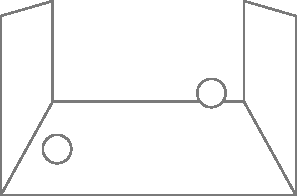
\includegraphics[width=\textwidth]{./graf/shadow_example_no_shadow.pdf}
        \caption{Shadowless scene, the positions of the spheres are ambiguous.}
        \label{fig:shadow_balls_no_shadow}
    \end{subfigure}
    \hfill
    \begin{subfigure}{0.4\textwidth}
        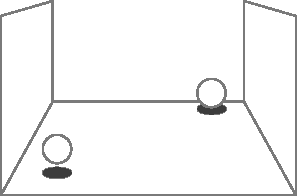
\includegraphics[width=\textwidth]{./graf/shadow_example_shadow_1.pdf}
        \caption{The upper ball seems placed on the surface.}
        \label{fig:shadow_balls_shadow_1}
    \end{subfigure}

    \begin{subfigure}{0.4\textwidth}
        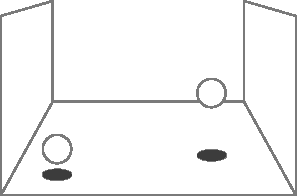
\includegraphics[width=\textwidth]{./graf/shadow_example_shadow_2.pdf}
        \caption{The upper ball seems to hover halfway.}
        \label{fig:shadow_balls_shadow_2}
    \end{subfigure}
    \hfill
    \begin{subfigure}{0.4\textwidth}
        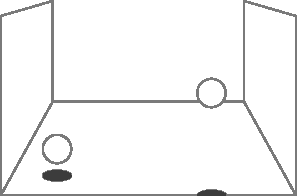
\includegraphics[width=\textwidth]{./graf/shadow_example_shadow_3.pdf}
        \caption{The upper ball seems high in the air and closer to the observer.}
        \label{fig:shadow_balls_shadow_3}
    \end{subfigure}
        
    \caption{The position and scale of the spheres do not change, yet the perceived locations in 3D space are dictated by the shadow.}
    \label{fig:shadow_balls_example}
\end{figure}
The importance of shadows for understanding the 3D composition of a scene is especially great when an observer is devoid of stereo visual information, such as in the case of observing an image displayed on a regular monitor. Shadows, lighting and perspective then become the sole sources of information about depth and the relative positions of objects in the scene.

These observations are also supported by a more recent 2018 review on the perception of shadows \cite{bib:article:shadow_perception}. It suggests more possible roles that shadows play in human perception of the world. Shadows help observers position objects in 3D space. Sometimes shadows are perceived as being a part of the object, so the lack of a shadow would make the object incomplete. Information about the shape of an object can also be derived from the shadow that it casts, as presented in Fig. \ref{fig:shadow_shape_example}.

\begin{figure}[h]
    \centering
    \begin{subfigure}{0.4\textwidth}
        
\includegraphics[width=\textwidth]{./graf/shadow_example_shadow_shape_1.pdf}
        \caption{The left shape could be a sphere, the right shape could be flat, like a coin.}
        \label{fig:shadow_shape_1}
    \end{subfigure}
    \hfill
    \begin{subfigure}{0.4\textwidth}
        
\includegraphics[width=\textwidth]{./graf/shadow_example_shadow_shape_2.pdf}
        \caption{The left shape could be a cube, and the right a shape with top and bottom faces not being parallel.}
        \label{fig:shadow_shape_2}
    \end{subfigure}

    \caption{The shadow can convey information on the shape of the object. It additionally describes whether an object is placed on a surface or above it.}
    \label{fig:shadow_shape_example}
\end{figure}

The review also mentions that shadows in art, even if depicted in a way that is impossible in the real world, are an important element for an image to be perceived as realistic and of high quality. This also applies to computer graphics, making rendering shadows a necessary element for any application that requires elevated realism or sophistication of the visual presentation. The difference between a scene with and without cast shadows is presented in Fig. \ref{fig:classroom_example} It is worth noting that since observers are not great at spotting physically incorrect shadows, as is stated in the studies, so graphics programmers can utilize this fact and take liberties with the realism of their shadows. This can lead to simplifying the algorithms producing them and improving their performance, with negligible impact on the apparent visual quality.

\begin{figure}
    \centering
    \begin{subfigure}{\textwidth}
        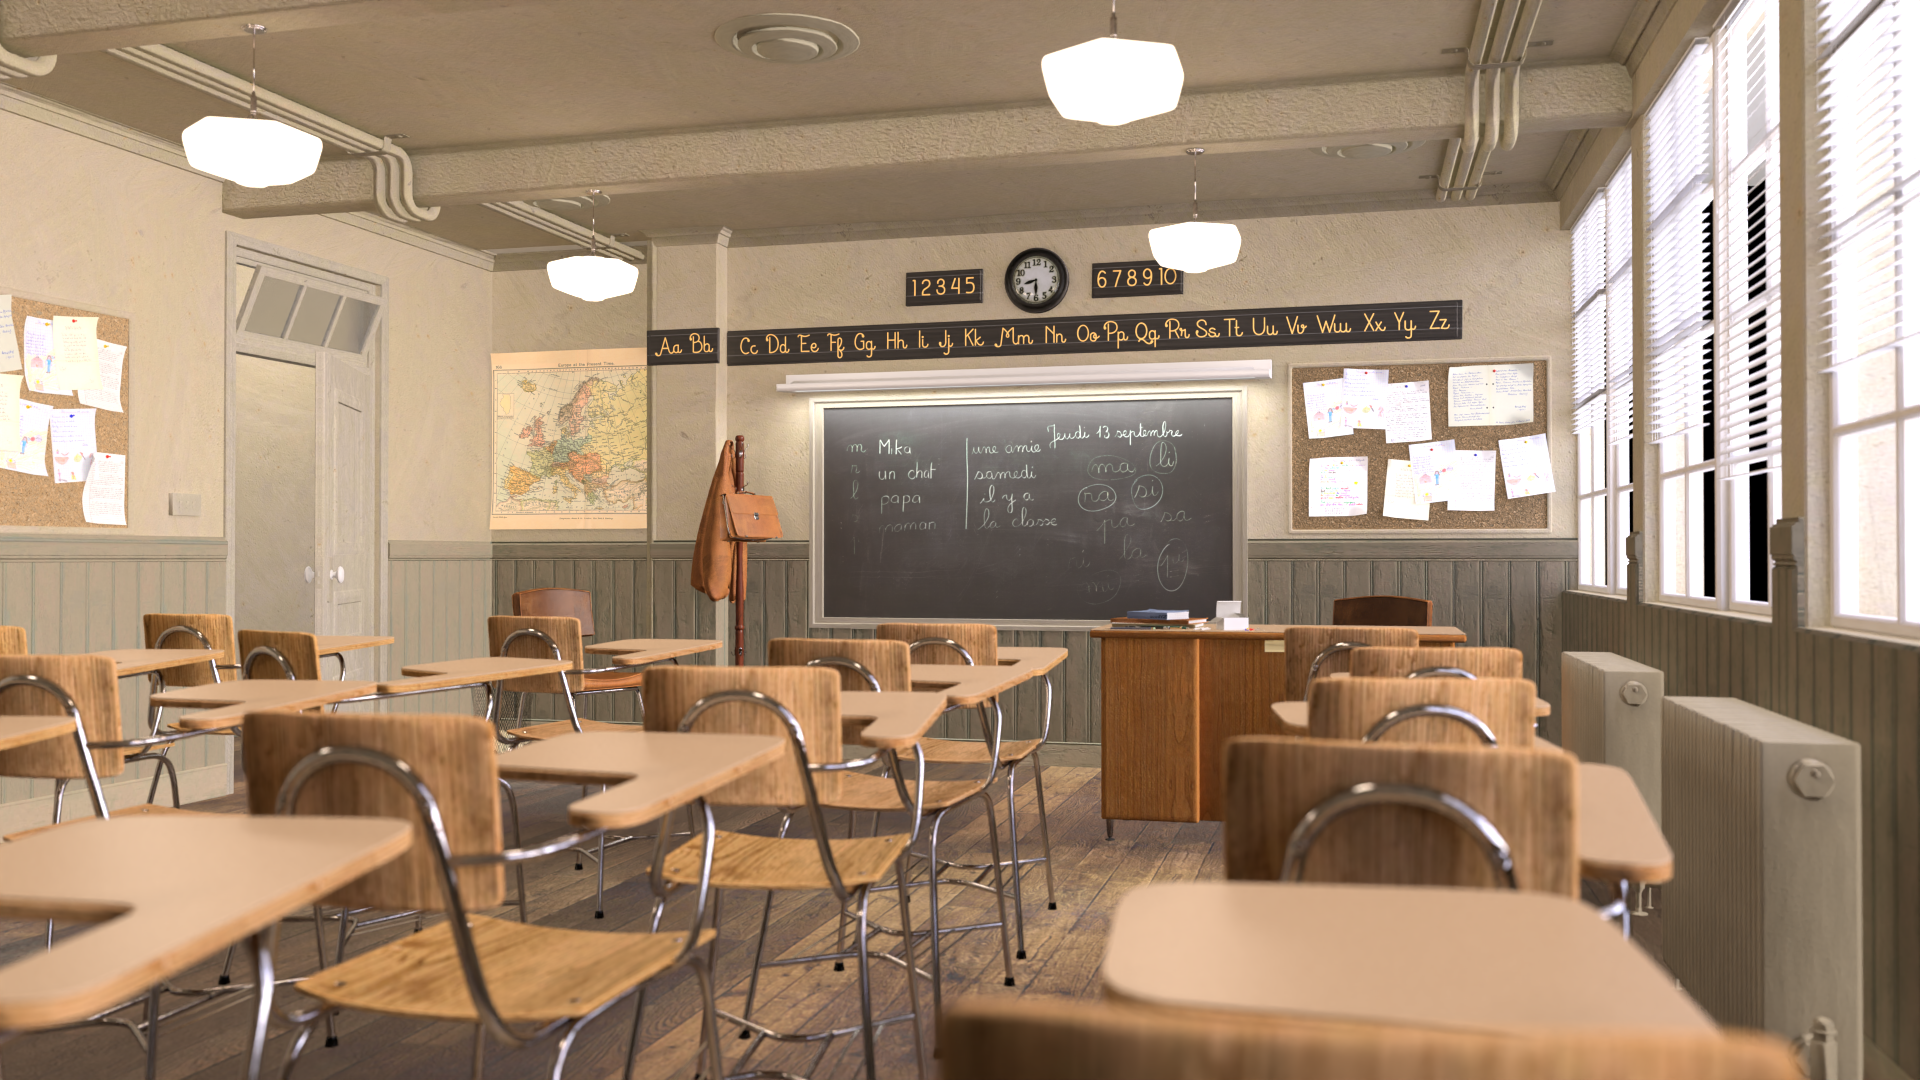
\includegraphics[width=\textwidth]{./graf/classroom_no_shadow.png}
        \caption{The scene rendered with no cast shadows, despite the high quality of models and materials, looks unrealistic and flat.}
        \label{fig:classroom_no_shad}
    \end{subfigure}

    \begin{subfigure}{\textwidth}
        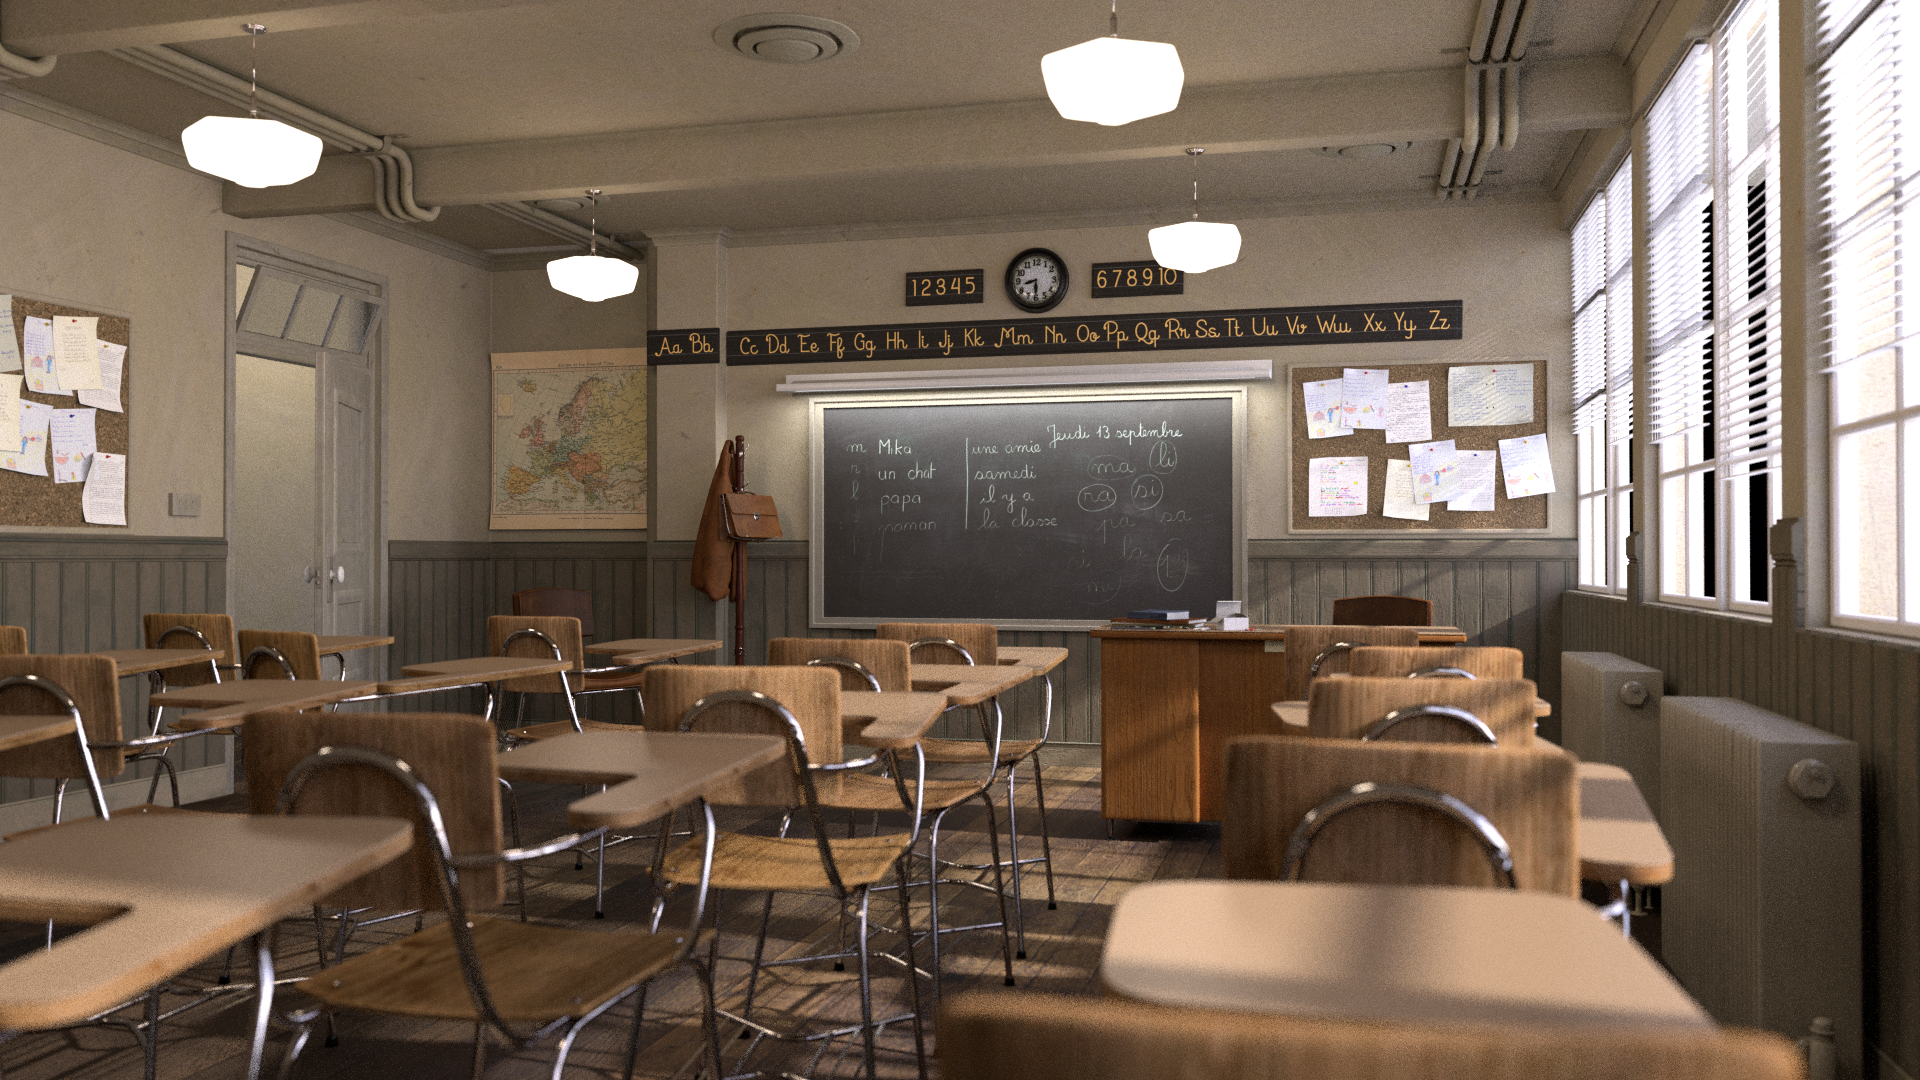
\includegraphics[width=\textwidth]{./graf/classroom_shadow.png}
        \caption{The scene rendered with cast shadows is realistic and reads well.}
        \label{fig:classroom_shad}
    \end{subfigure}

    \caption{The same scene rendered twice using Blender's Cycles renderer, with and without cast shadows. \textit{Scene source: ``Classroom'' by Christophe Seux, Blender demo files.}}
    % TODO: is this good enough for the source?
    \label{fig:classroom_example}
\end{figure}

\section{Shadow rendering techniques}

\subsection{Naming conventions}

In this thesis the term `shadows' is used interchangeably with term `cast shadows', not to be confused with shading on the surface of objects, which stems from the orientation of the surface with regard to the light source.

As presented in the ``Real-Time Rendering'' book \cite{bib:book:real_time_rendering}, a shadow is cast by a shadow caster, also called an occluder, onto a shadow receiver, when the caster occludes a line of sight from a point on the surface of the receiver to a light source.

Shadows can be differentiated into hard and soft shadows. Perfectly hard shadows are not observed in reality, as such a shadow would require an infinitely small light source. Hard shadows however are often found in computer-generated images, as they are relatively simple and cost-efficient to render. Soft shadows require more complex solutions, but enhance the realism of the rendered scene. A soft shadow, as shown in Fig. \ref{fig:shadow_soft} consists of an \textit{umbra}, being the fully shadowed region, and \textit{penumbra}, meaning the region that is partially in shadow. The appearance of a soft shadow, the sizes of the umbra and penumbra defining its softness, depend on the relative distances between the shadow caster, the shadow receiver, the light source and also the size of the light source.

\begin{figure}
    \centering
    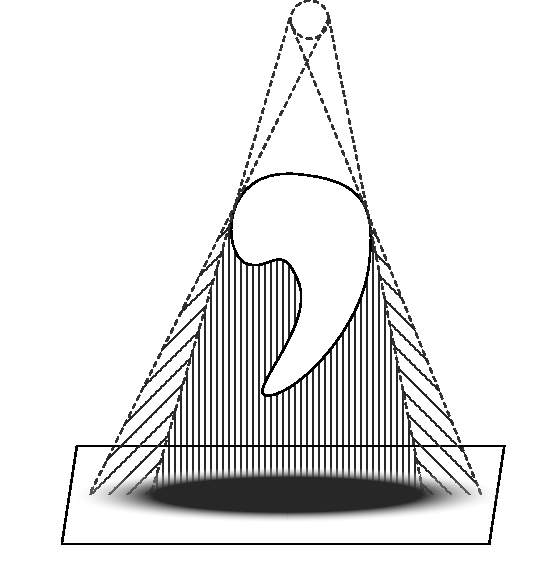
\includegraphics[width=0.5\textwidth]{./graf/shadow_example_soft.pdf}
    \caption{The umbra (under vertical lines) and penumbra (under slant lines) create a soft shadow.}
    \label{fig:shadow_soft}
\end{figure}

\subsection{Coarse distinction of shadow rendering techniques}

In this thesis a coarse distinction of the shadow rendering techniques is proposed, dividing them into three groups. The division is decided based on the main mechanism utilized in a technique. Additionally, techniques in each group share similar issues that researchers have attempted and are still attempting to resolve with newer iterations of the original algorithms.

The first group consists of shadow map-based, or image-based, techniques. They render the scene from the viewpoint of the light and store how far away scene geometry is in a depth buffer. This is then used when rendering the actual view of the scene to determine which parts are in shadow and which are lit. A common issue for these techniques is aliasing, which occurs when signals are sampled at different rates, causing artifacts. In the case of computer graphics, spatial aliasing is most often observed, where the source signal, being geometry, a texture, or a depth buffer as in the case of shadow mapping, is sampled in discrete locations in space at varying sample densities. It is not trivial to counteract aliasing in shadow map techniques and there are many approaches to solving this problem. On the other hand, it is relatively simple to achieve approximate soft shadows, with more advanced techniques allowing for more realistic results.

The second group contains geometry-based techniques. These approaches modify the scene geometry to create shadow volumes, which contain areas where light from a source does not fall. The shadow volumes are then rendered with a clever use of a stencil buffer, producing the information whether a surface point is in light or not. Such techniques suffer less aliasing problems than image-based ones, producing perfectly sharp shadow information on a per-pixel basis. They however introduce a lot of new geometry to the scene, the rendering time of which can be large and difficult to predict. It is also more difficult to achieve the effect of soft shadows with this approach.

The third group are ray-based techniques. They have only recently started being utilized in real-time scenarios, as they can be computationally costly and require powerful, modern hardware to run at interactive rates. This group of techniques is possibly the most intuitive, as it does not really rely on clever utilization of the rasterization hardware of a graphics card. To determine if a surface point is in shadow, a ray is cast in a straight line from the point to a light source. If any geometry is encountered along the ray, then the light source is occluded and the point is in shadow, otherwise it is lit. These techniques, apart from relying on powerful hardware, utilize specialized scene description data structures that accelerate these ray queries. They do not suffer from aliasing and can be extended to give photorealistic and physically-correct results.

The following sections introduce the techniques based on the publications which first described them. The sections attempt to mention them in logical order, highlighting the improvements and additions made to each group over the years. More detailed descriptions of the algorithms used to implement these methods will be given in chapter \ref{chapter:3_subject}. Additionally, the next section presents a now largely unused approach, that does not really fit into any of these categories, but is useful to build a geometric intuition of how shadows form.

\subsection{Planar shadows} \label{section:planar_shadows}
Planar shadows are one of the first techniques used for implementing shadow rendering and are not very robust, so they are mentioned in this thesis for historic reasons. They can be a help with understanding the geometry involved with shadows and their shape. That is because planar shadows are rendered using basic geometric projection.

Introduced by James Blinn in 1988 \cite{bib:article:blinn_shadows}, planar shadows are created by projecting the shadow caster onto a flat surface of the shadow receiver. The caster vertices are projected along a vector between the vertex and a light source onto a planar surface of the receiver. This is achieved with a projection matrix, which multiplied with the vertex positions of the caster gives a new mesh, flattened onto the planar surface. This mesh can then be rendered on top of the shadow receiver with a black material, giving the illusion of a shadow. The technique is described in more detail in section \ref{section:planar_shadows_impl}.

While very simple and intuitive, this approach has many shortcomings that nowadays render it obsolete. The application needs to keep track of shadow casters and receivers separately, to know which objects should be projected onto which surfaces. Issues occur when a light source is between the caster and receiver. In such a situation an incorrect anti-shadow is created, as the operation of projection through a point is still valid. The receivers have to be planes, and special care needs to be taken to only draw the shadow on top of a receiver. Since the shadow is a separate mesh, it could be rendered beyond the mesh of a receiver. Additionally, objects cannot shadow themselves. On the other hand planar shadows give a lot of artistic control over the appearance of shadows and even their shape, as they can be manipulated just as any other mesh.

\subsection{Basic Shadow Mapping}
\label{section:basic_mapping}
The general algorithm for shadow mapping was initially described by Lance Williams in 1978 in the article ``Casting curved shadows on curved surfaces'' \cite{bib:article:wiliams_curved_shadows}. The title immediately hints at the biggest strengths of this technique at the time: it is robust, allowing any scene objects to cast hard shadows onto others, regardless of their shapes and without the need for special treatment of casters and receivers as with planar shadows. In fact, similar shadow mapping techniques that utilized the z-buffer were already known before this article, but they could only be used for geometry consisting of planar polygons. This technique can be used to render shadows anywhere where any scene rendering can be obtained at all, which includes smooth, curved parametric surface patches.

The article presents the general method of shadow mapping, along with its advantages and disadvantages. The rationale of the technique is based on the fact that all surfaces `seen' by a light source from its point of view are lit by it, while all others are in shadow. To determine surface visibility for a light source, the scene is simply rendered from the viewpoint of the light source. This rendering is called the shadow map. Such an intermediate rendering, which will not be presented on screen but is only a step in the process of creating the final render of a scene, is often called a render pass. This rendering does not need to produce a color image, but only a depth- or z-buffer. This buffer is used in the standard rasterization pipeline to perform depth culling, so no special implementation is needed. Moreover, the existing highly optimized and hardware-supported rasterization architecture is utilized. The z-buffer stores the distances from the observer to the closest surface point in the scene per-texel. Once this view is obtained, the scene can be rendered again, in the usual manner from the point of view of the observer. When deciding whether a surface point is in shadow or not, the distance between the point and the light source can be calculated and compared to the value stored in the previously obtained shadow map. If the distance of the surface being rendered to the light source is greater than the depth read from the shadow map, then the surface is in shadow, and some other object that is closer to the light source occludes it. Otherwise, the surface is lit and further shading computations can take place, such as diffuse and specular lighting calculations.

Variants of shadow mapping have been described over the years, and techniques based on this approach are currently most widely utilized for real-time rendering. This is not surprising when considering the advantages of this method. The issues present in planar shadows such as the need to separate shadows casters and shadow receivers, difficulty casting shadows onto non-planar surfaces, impossibility of obtaining self-shadowing and possibility for shadows to appear in empty space beyond any receivers are all solved with shadow mapping. The technique is also relatively simple to implement and utilizes the rasterization pipeline in its full potential. The cost of the algorithm per light source is roughly twice the cost of rendering without shadow mapping, as scene objects need to be transformed and rendered into the z-buffer. The cost of rendering the shadow map will however be almost always less than rendering the scene, as there are no per-pixel lighting computations done to obtain color. In modern rendering pipelines the color render target buffer can be omitted altogether, making it also possible to not run the pixel shader at all.

% TODO: Do I want figures here or in the third chapter?

The disadvantages of shadow mapping are outweighed by its advantages, but are not trivial to combat. One disadvantage is that basic shadow mapping generates only hard shadows, which are not realistic and are prone to visible aliasing in the final image. Multiple specializations of this technique exist that make it possible to render soft shadows with varying levels of realism and correctness. Another significant issue is the fact that this technique introduces a second level of aliasing to the shadows. This is because the shadow map itself is an image representation of the scene, making it a discrete view of continuous scene geometry. This creates a few problems that need to be addressed. For one, numerical representation resolution errors can be introduced into the shadow map. This can be easily minimized by rendering into a 16-bit or more z-buffer and setting the near and far clipping planes of the shadow map view to tightly encompass the scene. The second problem being self-shadowing, also called surface-acne, is much more prominent and immediately observable in a naive implementation. As the samples of depth values stored in the shadow map are texels, they represent a non-zero area for a point location on a surface. When the exact depth values calculated when rendering the main view of the scene are compared with these spatially discretized samples, a surface can erroneously shadow itself, creating high-frequency, high-contrast patches of shadow, which often create intrusive moiré patterns on screen. This problem can be reduced by using a higher resolution shadow map, resulting in more dense depth sampling and decreasing the size of self-shadowing patches. This however is expensive and will not fully resolve the problem. Another method to deal with surface-acne is to use a depth bias when rendering the shadow map. A depth bias is a value that is added to the actual depth values before storing them in the z-buffer. By adding a positive depth bias, the depth of a surface can be pushed further away from the light source, under the actual surface. This way the actual distance between the light source and the surface being rendered in the final pass will always be less than the depth stored in the shadow map. This however can cause issues with light-leaking, or peter-panning, where contact shadows get detached from their casters. Methods to counteract this, as well as an example implementation will be shown in chapter \ref{section:basic_mapping_impl}. More issues with shadow mapping will be described in the following sections, along methods to circumvent them.

\subsection{Fitting shadow maps}
Here shadow map warping is described along with z-partitioning, aka cascaded shadow maps.

\subsection{Filtering shadow maps?}
There are many filtering techniques, so each should probably get its own subsection. PCF, variance shadow maps

\subsection{Rendering soft shadows with shadow maps}
Here techniques for obtaining soft shadows are described.

\subsection{Basic shadow volumes}
Here geometry/stencil based techniques begin, starting with stencil-based, hard-shadow, per-triangle shadow volumes.

%%%%%%%%%%%%%%%%%%%%%%%%%%%%%%%%%%%%%%%%%%%%%%%%%%%%%%%%%%%%%%%%%%%%%%%%%%%%%%%%

\begin{itemize}
\item What problem do I want (have to :-) to solve?
\item Why the problem is important?
\item How do others solve the problem?
\item What are pros and cons of my solution?
\end{itemize}

References to 
book \cite{bib:book},
scientific papers in journals \cite{bib:article},
conference papers \cite{bib:conference},
and web pages \cite{bib:internet}.

Equations should be numbered:
\begin{align}
y = \frac{\partial x}{\partial t}
\end{align}

\begin{itemize}
\item problem analysis, problem statement
\item state of the art, literature research (all sources in the thesis have to be referenced, eg journal article \cite{bib:article} book \cite{bib:book}, conference paper \cite{bib:conference}, internet source \cite{bib:internet})
\item description of known solutions, algorithms
\item location of the thesis in scientific domain
\item The title of this chapter is similar to the title of the thesis.
\end{itemize}

\begin{Definition}\label{def:definition}
body of the definitions
\end{Definition}

\begin{Theorem}[optional name]\label{t:theorem}
body of the theorem
\end{Theorem}

\begin{Example}[optional name]\label{ex:example}
body of the example
\end{Example}

%%%%%%%%%%%%%%%%%%%%%%%%


